\chapter{\textbf{Технологический раздел}}

\hfill

В соответствии с выбранной задачей -- реализация загружаемого модуля ядра для отслеживания USB-устройств, являющихся ключом для доступа к приложению. Необходимо выбрать средства реализации, создать модули и интерфейс, описать ограничения и порядок работы программы. 

\section{\textbf{Выбор технологий}}

Для реализации был выбран язык программирования C. Компилятор -- gcc. Для облегчения сборки был написан Makefile, позволяющий запускать сборку одной командой, листинг \ref{lst:makefile}.

\section{\textbf{Хранение данных }}

Параметры USB устройств, идентификатор поставщика и изделия, а также список секретных файлов и приложений хранятся в конфигурационном файле. Пример конфигурационного файла USB устройств представлен в листинге \ref{lst:config_usb}. Конфигурационный файл секретных файлов и приложений -- листинг \ref{lst:config_file}.

Пароль для доступа к зашифрованным данным хранится на разрешенном USB устройстве в файле \textit{password.txt}.

\section{\textbf{Загружаемый модуль}}

Цель работы создание загружаемого модуля, реализация загрузки и удаления представлена в листинге \ref{lst:module}.

После компиляции загружаемого модуля объектный файл может быть загружен в ядро с помощью команды \textit{insmod} с правами суперпользователя, для выгрузки используется команда \textit{rmmod}.

\section{\textbf{Функция-обработчик}}

В листинге \ref{lst:notify} представлена реализация функции обратного вызова добавления или удаления USB устройства \textit{static int notify(struct notifier\_block *self, unsigned long action, void *dev)}. 

С последующим вызовом, в зависимости от события \textit{static void usb\_dev\_remove(struct usb\_device *dev)}, \textit{static void usb\_dev\_insert(struct usb\_device *dev)}.

\section{\textbf{Проверка принадлежности устройства известным }}

Чтобы узнать можно ли расшифровать файл, необходимо узнать принадлежит ли устройство списку разрешенных устройств. Каждое устройство имеет уникальную пару идентификатор поставщика и идентификатор изделия, по ней и будет происходит поиск. Также в известных устройствах хранится файл с паролем для расшифровки секретных данных.

Реализация данной проверки представлена в листинге \ref{lst:check}.

Считывание пароля представлено в листинге \ref{lst:password}.

\section{\textbf{Проверка принадлежности устройства известным }}

После проверки принадлежности, при необходимости вызываются функции шифровки и расшифровки файлов, которые вызывают исполняемый файл пользовательского пространства.

Реализация этих функций представлена в листинге \ref{lst:user_call}.

\section{\textbf{Пример вывода в dmesg }}

На рисунке представлен пример работы загружаемого модуля.

\begin{figure}[H]
	\centering
	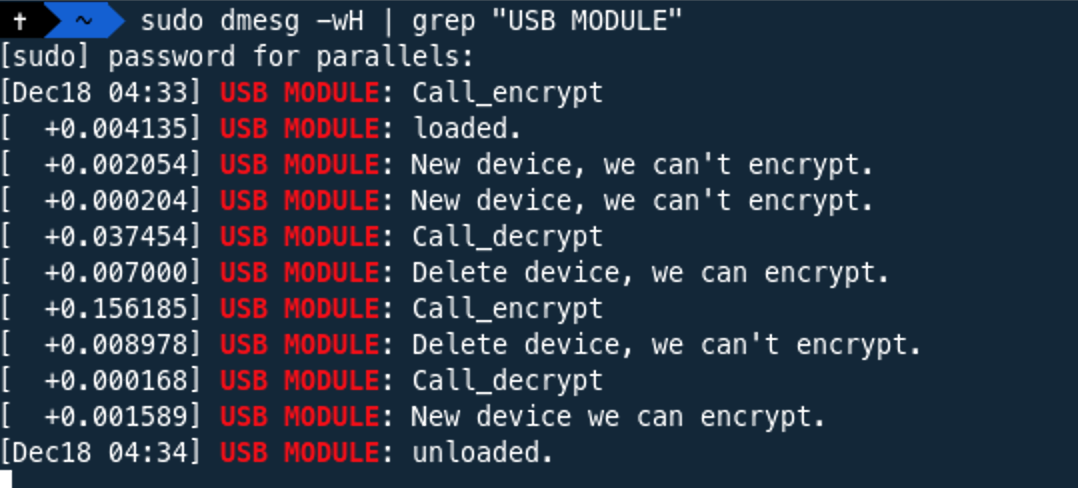
\includegraphics[scale=0.8]{example}
	\caption{Пример работы загружаемого модуля. }
	\label{img:example}
\end{figure}

\section{\textbf{Вывод}}

Реализовано спроектированное ПО, представлены результаты. 
